\section[Specyfika testowanych Urządzeń]{Specyfika testowanych Urządzeń}
Ze względu na ograniczenia związane ze zużyciem energii, urządzenia mobilne są nie często wykorzystywane do większych zadań obliczeniowych. Zwykle praca procesorów graficznych wykorzystywana jest głównie do wspierania aplikacji graficznych. Procesory Graficzne działają w modelu przetwarzania pojedynczą instrukcją kilku elementów pamięci (SIMD). Tak by móc jedną instrukcją w tym samym czasie wykonać operacje na przykład na kilku pixelach z obrazka. 
\begin{figure}[H]
	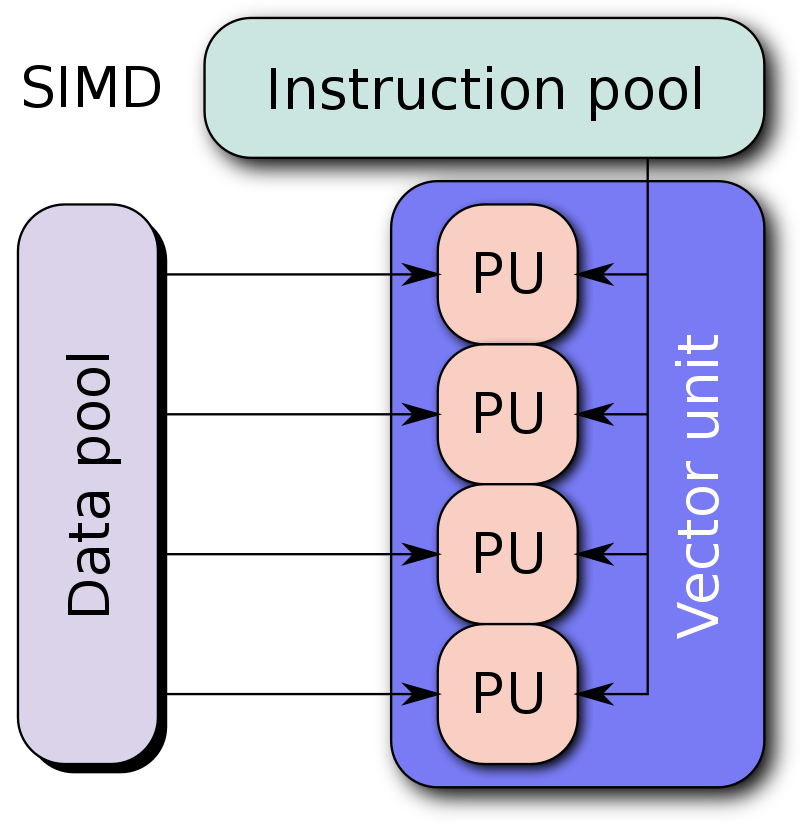
\includegraphics[scale=0.16]{imgs/SIMD2.svg.png}
	\caption{SIMD}
\end{figure}

\subsection[Porównanie Graficznych Procesorów Mobilnych]{Porównanie Graficznych Procesorów Mobilnych}
Dwoma głównymi producentami procesorów graficznych na mobilne platformy są Qualcomm produkujący procesory Adreno i ARM tworzący GPU o nazwie Mali. 
Oto podstawowe wady i zalety wymienionych produktów.
\begin{itemize}
	\item Adreno zalety:
	\begin{itemize}
		\item Lepszy Performance
		\item Wspiera nowsze Api
		\item Mniej się przegrzewa
	\end{itemize}
	\item Adreno wady:
	\begin{itemize}
		\item Droższy
		\item Mniej zoptymalizowany
		\item Słabszy przy renderowaniu.
	\end{itemize}
	\item Mali zalety:
	\begin{itemize}
		\item Bardziej rozpowszechnione, więc lepiej zoptymalizowane.
		\item Niższa cena
		\item Większe częstotliwości zegara
		\item Szybsze renderowanie.
	\end{itemize}
	\item Mali wady:
	\begin{itemize}
		\item Gorszy performance
		\item Gorszy support Api
		\item Bardziej się grzeje.
	\end{itemize}
\end{itemize}
	
	
\subsection[Urządzenia wykorzystane do testowania]{Urządzenia wykorzystane do testowania}
\subsubsection[Xiaomi Mi A2 Lite]{Xiaomi Mi A2 Lite}
Jest to telefon z lipca 2018 roku. Posiadający ośmiordzeniowy procesor Cortex A53, z częstotliwością zegara 2.0GHz. Pamięć systemowa urządzenia to 3GB. Umieszczono w nim Procesor graficzny Adreno 506. Procesor ten posiada 96 jednostek mogących jednocześnie wykonywać wątki na urządzeniu. Częstotliwość zegara procesora wynosi 650MHz. Dodatkowo posiada on 128 KB pamięci wbudowanej w chip GPU oraz 8KB, jest to pamięć typu LPDDR3 933MHz i przepustowości 7.4GB/s pamięć cache. Wspiera następujące API: Vulkan 1.0, OpenGL 3.2, DX11, OpenCL 2.0. Telefon Posiada system operacyjny Android w wersji 10. Sterownik OpenCL na urządzeniu jest w wersji \#7331a27 z 11/13/19, posiada wsparcie dla typu zmiennoprzecinkowe Half, oraz dla współdzielenia zasobów z OpenGL. Nie posiada wsparcia dla typów zmiennoprzecinkowych podwójnej precyzji Double.
\subsubsection[Huawei P20 Lite]{Huawei P20 Lite}
Jest to Urządzenie z marca 2018 roku. Wyposażone jest w 8 rdzeniowy procesor 4x2.36 GHz Cortex-A53 + 4x1.7 GHz Cortex-A53. Posiada on 4GB pamięci systemowej. Wbudowany procesor graficzny to Mali-T830 MP2, procesor posiada dwie jednostki wykonawcze. Wg danych producenta pojedyncza jednostka w tym procesorze może maksymalnie wykonywać 256 wątków. Częstotliwość zegara wynosi 650MHz, posiada 16KB pamięci cache, jest to pamięć LPDDR3 o częstotliwości 933MHz i przepustowości do 14.9 GB/s. Wspiera następujące Api: Vulkan 1.0, OpenCL 1.2, OpenGL 3.2. Wspiera typ Half oraz Double, nie wspiera współdzielenia zasobów z OpenGL. Telefon działa z systemem operacyjnym Android w wersji 8
\subsubsection[HTC Desire 820]{HTC Desire 820}
Telefon z 2014 roku, wyposażony w procesor ośmiordzeniowy 1,7 GHz quad-core Cortex-A53 + 1 GHz quad-core Cortex-A53. Posiada 2GB pamięci RAM. Posiada procesor graficzny Adreno 405. Gpu może wykonywać na raz 48 wątków, dodatkowo posiada 256KB pamięci dedykowanej. Wykorzystano pamięć typu LPDDR3 z częstotliwością 666.5MHz i szybkości 5.3GB/s Wspierane przez urządzenia Api to: OpenGL 3.2, OpenCL 1.2, DX11. Telefon Dla Systemu Android w wersji 5 posiada sterownik OpenCL w wersji z 29.04.15, a z androidem 6 w wersji z 23.03.2016. Wspiera typ Half, nie wspiera Double, możliwe do wykorzystania rozszerzenie współdzielenia zasobów między OpenCL i OpenGL.
\subsubsection[Xiaomi Redmi Note 7]{Xiaomi Redmi Note 7}
Telefon wydany na początku 2019 roku. Posiada procesor ośmiordzeniowy Qualcomm Kryo 260 z częstotliwością do 2,2 GHz. Wyposażony w 6GB pamięci systemowej. Dodatkowo posiada Procesor graficzny Adreno 512. GPU działa z częstotliwością 850MHz posiada 256KB pamięci dedykowanej i 16KB cache, pamięć typu LPDDR4 o częstotliwości 1866MHz i przepustowości do 29.8GB/s. Może wykonywać na raz 128 wątków. Telefon działa z systemem android w wersji 10, posiada sterownik OpenCL w wersji:\#9b15012 z 09/17/20.Wspiera Api Vulkan 1.0, OpenGL 3.2, DX11, OpenCL 2.0. OpenCL nie wspiera typu double, ale wspiera typ Half oraz współdzielenie zasobów z OpenGL.
\subsubsection[Samsung Galaxy A70]{Samsung Galaxy A70}
To urządzenie, którego premiera odbyła się na początku 2019 roku. wyposażony w procesor ośmiordzeniowy Kryo 460 z częstotliwością zegara do 2 GHz. Posiada 6GB pamięci RAM. Dodatkowo posiada procesor graficzny Adreno 612 o częstotliwości 845Mhz, 128 wątkach, wbudowanej pamięci 256KB i 16KB pamięci cache, jest to pamięć typu LPDDR4X o częstotliwości 1866MHz i przepustowości do 14.9GB/s. Android w wersji 10 ze sterownikiem OpenCL w wersji \#e1ac91e z 11/17/20. Wspiera typ Half, nie wspiera Double, możliwe do wykorzystania rozszerzenie współdzielenia zasobów między OpenCL i OpenGL.
\subsubsection[Porównanie]{Porównanie}
Zdecydowanie urządzeniem z najsłabszymi parametrami jest HTC Desire 820. Xiaomi Mi A2 Lite oraz Huawei P20 lite posiadają konkurencyjne parametry, jednak są urządzeniami posiadające podzespoły od różnych producentów. Najmocniejszymi są Redmi Note 7, który ma najszybszą pamięć oraz najszybciej pracujący procesor, oraz SAmsung Galaxy A70, który ma najnowszy procesor graficzny.



